% =====================================================================
% AegisBench, IEEE Geoscience and Remote Sensing Letters submission.
%
% Uses the official IEEEtran.cls V1.8b shipped in the IEEE Transactions
% LaTeX2e author kit (a copy sits beside this file). GRSL enforces a
% five-page limit; check the page count on every edit.
%
%   pdflatex aegisbench_grsl && bibtex aegisbench_grsl && \
%   pdflatex aegisbench_grsl && pdflatex aegisbench_grsl
%
% Review is single blind, so author names and affiliation stay in.
% Do NOT run the anonymization scanner on this document; that machinery
% belongs to the double-blind WACV version only.
%
% Every number below is read from a file in results/. The extraction is
% reproducible: scripts/grsl_figures.py builds both figures from the same
% CSVs. Do not edit a number here without changing its source.
% =====================================================================
\documentclass[journal]{IEEEtran}

\usepackage{amsmath}
\usepackage{graphicx}
\usepackage{booktabs}
\usepackage{cite}
\usepackage{url}

\hyphenation{HERIDAL VisDrone Kosch-mieder}

\begin{document}

\title{AegisBench: Aerial Search-and-Rescue Person\\Detection Under Physically Modeled\\Atmospheric Degradation}

\author{Prem~Kamasani and Amogh~Vinaykumar%
\thanks{The authors are with Flower Mound High School, Flower Mound, TX 75028 USA (e-mail: altisorbital@gmail.com).}%
\thanks{The benchmark code, corruption engine, and evaluation pipeline are available at \protect\url{https://github.com/Altis-2026/AegisBench}. No imagery is redistributed; every corrupted image regenerates bit-identically from the source datasets.}}

\markboth{IEEE Geoscience and Remote Sensing Letters}%
{Kamasani \MakeLowercase{\textit{and}} Vinaykumar: Aerial Search-and-Rescue Detection Under Physically Modeled Atmospheric Degradation}

\maketitle

\begin{abstract}
Aerial person detection supports land search and rescue, but the airborne
imagery used to benchmark it is acquired in clear air and good light,
whereas the missions that need it are flown into smoke, dust, rain, and
darkness. We quantify the resulting gap. AegisBench applies nine
corruptions derived from documented radiative transfer and sensor models,
including Koschmieder scattering for the smoke and dust families and a
linear-domain photometric model for illumination loss, at three severities
each calibrated against a declared and machine-checked image statistic.
Three architecturally distinct detectors are evaluated across 168
conditions on two airborne datasets spanning the high- and low-altitude
regimes, scored by one evaluator at operating points frozen on
clear-condition validation data. Degradation is strongly
condition-dependent: at the highest severity, rain costs YOLOv11 only 3.6
points of recall on low-altitude imagery but removes almost all of it at
high altitude. Illumination loss is the one universal failure. At 4.5
stops of exposure loss, recall reaches exactly 0.000 for all three
detectors on both datasets, all 1000 bootstrap resamples agree, and
mAP$_{50}$ falls to at most 0.010, confirming the collapse independently
of any confidence threshold. Two corruptions matched to within 3\% in mean
optical depth differ 6.7-fold in cost, so the loss is not reducible to
contrast reduction alone. An unmodified detector run on real night imagery
from an unrelated airborne benchmark recovers 2 of 128 annotated persons,
consistent with the modeled result.
\end{abstract}

\begin{IEEEkeywords}
Aerial imagery, atmospheric scattering, benchmark, low-light imaging,
object detection, robustness, search and rescue, unmanned aerial vehicles.
\end{IEEEkeywords}

% ---------------------------------------------------------------------
\section{Introduction}
% ---------------------------------------------------------------------

\IEEEPARstart{A}{irborne} optical imaging of the land surface is
governed by the atmosphere between the sensor and the ground. Scattering
and absorption by aerosols attenuate scene radiance and add path
radiance, and the available illumination sets the photon flux the sensor
integrates. Both effects are routinely modeled in remote sensing, and
both are treated as nuisances to be corrected before analysis. When the
analysis is automated person detection for land search and rescue, they
stop being nuisances and become the operating condition. A search flight
is launched because something has gone wrong on the ground, which is
frequently the same event that fills the air with smoke or dust, or that
leaves responders working after sunset.

The imagery used to develop and benchmark aerial person detectors does
not reflect this. HERIDAL~\cite{bozic2019heridal} and
SARD~\cite{sambolek2021sard}, the two standard datasets for the task,
were both acquired in clear air and good light, and detectors trained on
them report strong accuracy under those conditions. What happens to that
accuracy when optical depth rises or illumination falls is, at present,
not measured. For a capability whose failures are missed rescues, the
absence of that measurement is itself the problem.

This letter supplies it. We construct nine corruptions of airborne
optical imagery from documented radiative transfer and sensor models
rather than from generic image-processing filters, calibrate each to a
declared and machine-checked image statistic, and evaluate three
architecturally distinct detectors across all resulting conditions on
both datasets. Three properties separate this from a transplant of the
common-corruptions
methodology~\cite{hendrycks2019imagenetc,michaelis2019benchmarking} into
aerial imagery. First, the corruption parameters are physical quantities,
so a severity level corresponds to a stated optical depth or a stated
exposure loss rather than to an arbitrary index. Second, severity is
verified against a measured image statistic instead of chosen by
inspection. Third, each detector's confidence threshold is fixed once on
clear-condition validation data and held across every degraded condition,
which is the constraint a deployed system actually operates under.

Robustness benchmarking for airborne imagery under degraded conditions is
recent and partial. UAV-C~\cite{liu2024uavc} evaluates UAV tracking, not
detection, against generic corruptions. HazyDet~\cite{feng2024hazydet}
pairs physics-driven synthetic haze with real hazy drone photographs,
covering one condition and general object categories rather than persons.
WRRT-DETR~\cite{liu2025wrrtdetr} builds a weather-robust detector around
a maritime dataset. Each addresses a different task, a narrower set of
conditions, or a different surface. None measures how aerial
search-and-rescue person detection degrades as a function of a physical
atmospheric or radiometric parameter, which is what we report.

% ---------------------------------------------------------------------
\section{Corruption Models}
% ---------------------------------------------------------------------

Nine corruptions are grouped into four families by the disaster
environment they represent: flood (\texttt{water\_glare},
\texttt{turbidity\_cast}, \texttt{inundation}), wildfire
(\texttt{smoke\_haze}, \texttt{fire\_warm\_tint}), storm
(\texttt{rain\_streaks}, \texttt{motion\_blur}, \texttt{low\_light}), and
earthquake or post-disaster dust (\texttt{dust\_haze}).
Table~\ref{tab:taxonomy} lists each with its optical mechanism and
calibration statistic.

\subsection{Atmospheric Scattering}

The three haze corruptions follow the Koschmieder
model~\cite{koschmieder1924theorie,narasimhan2002vision} used throughout
atmospheric correction,
\begin{equation}
I(x) = J(x)\,t(x) + A\,\bigl(1 - t(x)\bigr),
\label{eq:koschmieder}
\end{equation}
where $J$ is clear-scene radiance, $A$ is airlight, and $t$ is
transmission. Severity is set by the mean transmission $\bar{t}$, so each
level corresponds to a mean optical depth $\tau = -\ln \bar{t}$
(Table~\ref{tab:taxonomy}). Transmission is spatially varying rather than
constant, generated as a band-limited noise field, since haze over
terrain is not uniform across a frame.

\texttt{smoke\_haze} and \texttt{dust\_haze} differ principally in
airlight chromaticity, neutral gray for combustion aerosol against brown
for suspended mineral particulate, and in the spatial structure of $t$.
Dust uses twice the transmission variance of smoke ($0.30$ against
$0.15$) at a finer base resolution (8 against 3 octave cells), plus
low-amplitude granular noise representing near-lens particulates.
\texttt{fire\_warm\_tint} applies (\ref{eq:koschmieder}) with a warm
airlight and a white-balance shift toward orange, modeling low
color-temperature firelight through smoke.

\subsection{Illumination Loss}

\texttt{low\_light} is modeled in the approximately linear photometric
domain~\cite{chen2018dark}. The image is linearized with a decode gamma
of 2.2, scaled by a photon gain $g$, shifted toward twilight
chromaticity, and returned through the inverse gamma with
signal-dependent shot noise and additive read noise whose relative
magnitude grows as $g$ falls. Severity is set by $g$, so each level
corresponds to an exposure loss of $\log_2 g$ stops: $-1.60$, $-2.94$,
and $-4.47$ for severities 1 through 3. This is the parameter against
which the headline result is plotted in Fig.~\ref{fig:lowlight}.

The remaining corruptions are not atmospheric processes.
\texttt{rain\_streaks} follows the directional streak model of Garg and
Nayar~\cite{garg2007rain} over a blurred veil, \texttt{motion\_blur}
models wind-induced platform shake, \texttt{turbidity\_cast} blends
toward a mud chromaticity and compresses contrast, \texttt{inundation}
alpha-blends semi-transparent standing water under a smooth mask, and
\texttt{water\_glare} adds specular sun-glint saturation.

\subsection{Calibration and Determinism}

Each corruption declares a measurable image statistic whose subset mean
must move monotonically across severities, verified on a fixed random
20-image subset of the HERIDAL test split held constant across all
corruptions and severities. Eight of nine pass directly.
\texttt{rain\_streaks} does not: streak density has no closed-form image
measure, and the substituted edge-strength proxy is confounded, since
added streaks raise measured edge strength while the veil blur applied in
the same corruption suppresses it. Its severity is instead set by its
generation parameters, which increase by construction. Recall still
degrades monotonically with it (Fig.~\ref{fig:spectrum}), independent
evidence that the corruption intensifies where this one proxy does not
track it.

The calibration statistic makes a severity ladder falsifiable within a
corruption. It is not a cross-corruption difficulty normalizer, and we
make no such claim. \texttt{smoke\_haze} and \texttt{dust\_haze}
illustrate the point: they reach $\tau = 1.386$ and $\tau = 1.427$ at
severity 3, matched to within 3\%, and nearly identical RMS contrast
(0.0475 against 0.0489), yet differ 6.7-fold in recall cost
(Section~\ref{sec:results}).

All pixel-unit parameters are specified per 1000 pixels of the longer
image side and scaled at runtime, so a severity means the same thing on a
$4000 \times 3000$ frame and a $640 \times 640$ frame. Corruptions are
appearance-only and do not displace object content, so clear-condition
ground-truth boxes stay valid; the exception is \texttt{inundation},
whose refraction ripple reaches about 1.4 pixels at severity 3 on a
4000-pixel frame, well below person scale. Every stochastic element is
seeded by a SHA-256 hash of the image identifier, corruption, severity,
and global seed, so the degraded benchmark regenerates bit-identically on
any machine.

% ---------------------------------------------------------------------
\section{Data and Evaluation Protocol}
% ---------------------------------------------------------------------

\subsection{Datasets}

HERIDAL~\cite{bozic2019heridal} is high-altitude orthophoto-scale
wilderness imagery at $4000 \times 3000$ pixels; we use its official
101-image test split, with 1391 training and 155 validation images
carved deterministically from the official training split. For
SARD~\cite{sambolek2021sard}, lower-altitude drone video of staged
rescue scenarios, we use a public re-export resized to $640 \times 640$
(4033 training, 860 validation, 862 test images). SARD frames originate
from video, so temporally adjacent frames are near-duplicates. Splitting
is group-aware, assigning every image sharing a filename token to exactly
one split, and we verified directly that no group appears in more than
one. The two datasets bracket the capture regimes in which this task is
flown.

\subsection{Detectors and Training}

We fine-tune Faster R-CNN~\cite{ren2015fasterrcnn}, a two-stage CNN,
YOLOv11~\cite{ultralytics2024yolo11}, a single-stage CNN, and
RT-DETR~\cite{zhao2024rtdetr}, a transformer detector, from pretrained
weights, one run per model per dataset, all at 1024-pixel input and seed
17. Faster R-CNN trains 26 epochs at learning rate 0.005, YOLOv11 80
epochs at 0.01, and RT-DETR 80 epochs at 0.0001, following each
architecture's established practice rather than a shared schedule.
Degraded data enters neither training nor threshold selection. Training
used a single 8-GB consumer GPU, so the benchmark is reproducible without
a cluster.

\subsection{Protocol}

Each detector's confidence threshold is selected once per dataset by
maximizing F1 on clear-condition validation data and frozen across all 28
conditions: 0.99 and 0.96 for Faster R-CNN on HERIDAL and SARD, 0.65 and
0.60 for RT-DETR, 0.45 and 0.30 for YOLOv11. Re-tuning per condition
would measure a best case unavailable to a system that must commit to a
threshold before a flight. All three architectures are scored by one
evaluator using greedy score-ordered matching at IoU $\geq 0.5$, one
prediction per ground-truth box, so no detector is scored by its own
framework's metric.

Both datasets pass through the same tiled inference
pipeline~\cite{akyon2022sahi} with 1024-pixel tiles and 256-pixel
overlap: a HERIDAL frame splits into 20 overlapping tiles, a SARD frame
passes through whole. Predictions are mapped back to full-image
coordinates and merged with class-agnostic non-maximum suppression, so
evaluation is always against full-resolution ground truth. Corruptions
are applied before tiling, since haze gradients and flood masks are
spatially coherent across a scene. Confidence intervals are bootstrap
percentiles over 1000 resamples of the test set by
image~\cite{efron1993bootstrap}, and every result row logs the commit, a
hash of the corruption configuration, the seed, and a timestamp.

\begin{table*}[!t]
\caption{The Nine Corruptions, Their Optical Mechanism, and the Statistic Defining Each Severity Ladder}
\label{tab:taxonomy}
\centering
\footnotesize
\begin{tabular}{llllrrr}
\toprule
Corruption & Family & Optical mechanism & Calibration statistic & s1 & s2 & s3 \\
\midrule
\texttt{water\_glare}     & Flood      & Specular sun-glint saturation            & saturated fraction $\uparrow$ & 0.0116 & 0.0182 & 0.1895 \\
\texttt{turbidity\_cast}  & Flood      & Sediment-laden water, contrast loss      & RMS contrast $\downarrow$     & 0.1098 & 0.0701 & 0.0378 \\
\texttt{inundation}       & Flood      & Semi-transparent standing water          & occluded fraction $\uparrow$  & 0.0830 & 0.2235 & 0.3921 \\
\midrule
\texttt{smoke\_haze}      & Wildfire   & Koschmieder, gray airlight ($\tau$ 0.36/0.80/1.39) & RMS contrast $\downarrow$ & 0.1170 & 0.0776 & 0.0475 \\
\texttt{fire\_warm\_tint} & Wildfire   & Low-CCT firelight through warm haze      & red/blue ratio $\uparrow$     & 1.6743 & 2.0721 & 2.4516 \\
\midrule
\texttt{rain\_streaks}    & Storm      & Directional streaks over a rain veil     & generation parameters$^{\dagger}$ & --- & --- & --- \\
\texttt{motion\_blur}     & Storm      & Wind-induced platform shake              & edge strength $\downarrow$    & 0.0764 & 0.0572 & 0.0472 \\
\texttt{low\_light}       & Storm      & Photon scaling ($-1.6/-2.9/-4.5$ stops) & mean luminance $\downarrow$  & 0.2355 & 0.1533 & 0.1175 \\
\midrule
\texttt{dust\_haze}       & Earthquake & Koschmieder, brown airlight ($\tau$ 0.43/0.87/1.43) & RMS contrast $\downarrow$ & 0.1094 & 0.0720 & 0.0489 \\
\bottomrule
\end{tabular}

\vspace{2pt}
\raggedright\footnotesize
Arrows give the required direction as severity increases. Values are
means over a fixed random 20-image subsample of the HERIDAL test split,
held constant across all corruptions and severities, and monotonicity is
checked automatically on these means. Mean optical depth
$\tau = -\ln\bar{t}$ and exposure loss $\log_2 g$, given in parentheses
for the three severities, are derived from the declared generation
parameters rather than measured from the imagery.
$^{\dagger}$\,\texttt{rain\_streaks} has no closed-form image statistic
isolating streak density, so its severity is set by its generation
parameters (streaks per megapixel, streak length, veil intensity, all
increasing by construction).
\end{table*}

% ---------------------------------------------------------------------
\section{Results}
\label{sec:results}
% ---------------------------------------------------------------------

\subsection{Clear-Condition Baselines}

The top row of Table~\ref{tab:severity3} gives clear-condition recall.
Precision is 0.855 to 0.903 on HERIDAL and 0.955 to 0.972 on SARD, and
mAP$_{50}$ is 0.785 to 0.835 and 0.896 to 0.929 respectively. On HERIDAL
these sit modestly below the commonly cited YOLOv5L reference of about
0.90 precision and 0.893 recall~\cite{bozic2019heridal} and are
comparable in precision and mAP; broad agreement across different
architectures and input pipelines is the claim, not superiority. Recall
is higher on SARD than on HERIDAL, consistent with lower-altitude capture
and larger relative object size. Because the two datasets do not share a
difficulty floor, degradation is read against each model's own baseline.

\subsection{Degradation Is Condition-Dependent}

Table~\ref{tab:severity3} reports recall at severity 3 for every
corruption, detector, and dataset. The spread is the central
observation. On SARD, \texttt{rain\_streaks} costs YOLOv11 3.6 points of
recall (0.891 to 0.855) while \texttt{low\_light} removes all of it. The
same corruption behaves differently across capture regimes:
\texttt{rain\_streaks} and \texttt{motion\_blur} are nearly harmless at
low altitude but remove essentially all recall at high altitude, where
persons subtend far fewer pixels and a streak or a blur kernel of the
same physical scale covers a larger fraction of the target. A single
averaged robustness score would hide both effects.

Fig.~\ref{fig:spectrum} shows the severity progression for YOLOv11 on
SARD. The ordering is not predicted by the calibration statistics.
\texttt{smoke\_haze} and \texttt{dust\_haze} arrive at severity 3 with
mean optical depths within 3\% of each other and RMS contrast within
3\%, yet recall differs 6.7-fold (0.391 against 0.058). We hypothesize
that the difference is carried by the spatial structure of the
transmission field rather than by its mean: dust uses twice the
transmission variance at a finer base resolution, so it disrupts the
high-spatial-frequency content that defines a small aerial target, while
smoke mostly lowers global contrast. This is a hypothesis. The present
data establish the discrepancy but do not isolate whether airlight
chromaticity, transmission granularity, or added grain carries it, which
requires an ablation we have not run.

\begin{table*}[!t]
\caption{Recall at Severity 3 for Every Corruption, Detector, and Dataset}
\label{tab:severity3}
\centering
\footnotesize
\begin{tabular}{llcccccc}
\toprule
& & \multicolumn{3}{c}{HERIDAL ($n=101$)} & \multicolumn{3}{c}{SARD ($n=862$)} \\
\cmidrule(lr){3-5}\cmidrule(lr){6-8}
Corruption & Family & Faster R-CNN & RT-DETR & YOLOv11 & Faster R-CNN & RT-DETR & YOLOv11 \\
\midrule
\emph{clear condition}    & ---        & 0.745 & 0.792 & 0.769 & 0.879 & 0.888 & 0.891 \\
\midrule
\texttt{water\_glare}     & Flood      & 0.614 & 0.682 & 0.653 & 0.629 & 0.646 & 0.666 \\
\texttt{turbidity\_cast}  & Flood      & 0.024 & 0.042 & 0.163 & 0.180 & 0.074 & 0.191 \\
\texttt{inundation}       & Flood      & 0.326 & 0.472 & 0.398 & 0.489 & 0.459 & 0.495 \\
\texttt{smoke\_haze}      & Wildfire   & 0.148 & 0.320 & 0.407 & 0.303 & 0.319 & 0.391 \\
\texttt{fire\_warm\_tint} & Wildfire   & 0.401 & 0.086 & 0.145 & 0.407 & 0.118 & 0.099 \\
\texttt{rain\_streaks}    & Storm      & 0.003 & 0.003 & 0.056 & 0.778 & 0.840 & 0.855 \\
\texttt{motion\_blur}     & Storm      & 0.000 & 0.000 & 0.003 & 0.398 & 0.329 & 0.478 \\
\texttt{low\_light}       & Storm      & \textbf{0.000} & \textbf{0.000} & \textbf{0.000} & \textbf{0.000} & \textbf{0.000} & \textbf{0.000} \\
\texttt{dust\_haze}       & Earthquake & 0.098 & 0.071 & 0.104 & 0.160 & 0.050 & 0.058 \\
\bottomrule
\end{tabular}

\vspace{2pt}
\raggedright\footnotesize
Recall at each model's frozen operating point, selected on
clear-condition validation data only. \texttt{low\_light} is the sole
corruption reaching exactly zero for every detector on both datasets.
\texttt{rain\_streaks} and \texttt{motion\_blur} separate the two capture
regimes most sharply, costing little at low altitude and nearly all
recall at high altitude.
\end{table*}

\begin{figure}[!t]
\centering
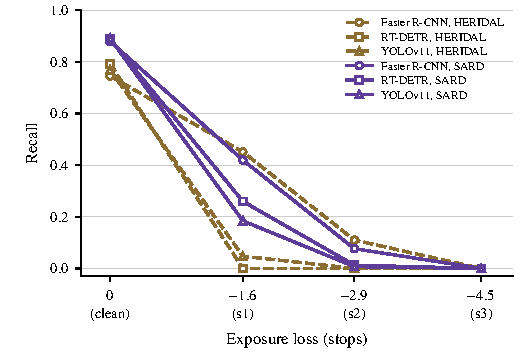
\includegraphics{figures/lowlight_collapse.pdf}
\caption{Recall against exposure loss under \texttt{low\_light}, plotted
against the physical drive parameter rather than a severity index. All
six detector and dataset combinations reach exactly zero recall by
$-4.47$ stops. Dashed lines are HERIDAL, solid lines SARD.}
\label{fig:lowlight}
\end{figure}

\begin{figure}[!t]
\centering
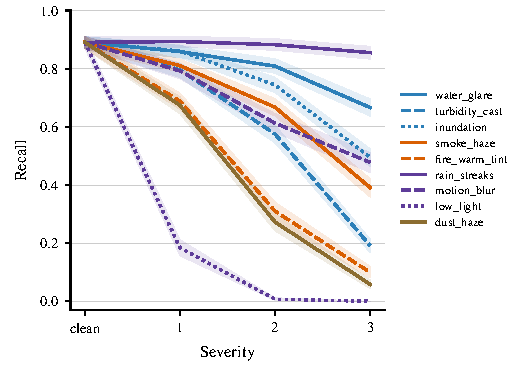
\includegraphics{figures/spectrum_sard_yolo11.pdf}
\caption{Recall against severity for all nine corruptions, YOLOv11 on
SARD, with bootstrap 95\% intervals shaded. Colour indicates disaster
family, line style distinguishes corruptions within a family. All curves
begin at the same clear-condition baseline.}
\label{fig:spectrum}
\end{figure}

\subsection{Illumination Loss Produces Total Failure}

\texttt{low\_light} is the one corruption that behaves the same way
everywhere. Table~\ref{tab:lowlight} and Fig.~\ref{fig:lowlight} give the
result: by $-4.47$ stops, recall is exactly 0.000 for all three
detectors on both datasets, and all 1000 bootstrap resamples agree, so
the interval is degenerate at $[0.000, 0.000]$. A two-stage CNN, a
single-stage CNN, and a transformer detector are about as
architecturally different as detectors get, and all three sit at the same
floor, which rules out an architecture-specific explanation.

A frozen-threshold zero could in principle reflect a badly placed
operating point rather than absent detections. mAP$_{50}$ settles this,
because it scans every threshold. It collapses in step with recall
(Table~\ref{tab:lowlight}): across all six detector and dataset pairs at
severity 3, mAP$_{50}$ is at most 0.010, against clear-condition values
of 0.785 to 0.929. If this were a calibration artifact, mAP would stay
high while recall fell. It does not, so the detections are absent rather
than merely below threshold.

Two statements hold on both datasets. Total failure by $-4.47$ stops
replicates for all three architectures, and Faster R-CNN is consistently
the most robust at every severity where any model retains recall, despite
carrying the strictest threshold (0.99 on HERIDAL against 0.65 and 0.45),
which rules out threshold strictness as the explanation. One statement
does not hold: RT-DETR loses all recall at every severity on HERIDAL,
including the mildest, but outperforms YOLOv11 at severities 1 and 2 on
SARD. That ordering is dataset-dependent, not an architecture property,
and we report it as such.

\begin{table*}[!t]
\caption{Detection Under Illumination Loss: Recall at the Frozen Operating Point and Threshold-Independent mAP$_{50}$}
\label{tab:lowlight}
\centering
\footnotesize
\begin{tabular}{llccccccc}
\toprule
& & & \multicolumn{3}{c}{Recall [bootstrap 95\% interval]} & \multicolumn{3}{c}{mAP$_{50}$} \\
\cmidrule(lr){4-6}\cmidrule(lr){7-9}
Model & Dataset & Thr. & $-1.60$ stops & $-2.94$ stops & $-4.47$ stops & $-1.60$ & $-2.94$ & $-4.47$ \\
\midrule
Faster R-CNN & HERIDAL & 0.99 & 0.451 [0.365, 0.540] & 0.110 [0.064, 0.163] & \textbf{0.000 [0.000, 0.000]} & 0.537 & 0.176 & 0.010 \\
RT-DETR      & HERIDAL & 0.65 & 0.000 [0.000, 0.000] & 0.000 [0.000, 0.000] & \textbf{0.000 [0.000, 0.000]} & 0.001 & 0.000 & 0.000 \\
YOLOv11      & HERIDAL & 0.45 & 0.048 [0.027, 0.073] & 0.000 [0.000, 0.000] & \textbf{0.000 [0.000, 0.000]} & 0.064 & 0.000 & 0.000 \\
\midrule
Faster R-CNN & SARD    & 0.96 & 0.419 [0.389, 0.452] & 0.077 [0.060, 0.094] & \textbf{0.000 [0.000, 0.000]} & 0.546 & 0.142 & 0.000 \\
RT-DETR      & SARD    & 0.60 & 0.260 [0.233, 0.288] & 0.013 [0.007, 0.019] & \textbf{0.000 [0.000, 0.000]} & 0.421 & 0.049 & 0.001 \\
YOLOv11      & SARD    & 0.30 & 0.184 [0.157, 0.212] & 0.007 [0.003, 0.012] & \textbf{0.000 [0.000, 0.000]} & 0.247 & 0.018 & 0.000 \\
\bottomrule
\end{tabular}

\vspace{2pt}
\raggedright\footnotesize
Exposure loss in stops is $\log_2 g$ for the declared photon gain $g$,
corresponding to severities 1 through 3. Recall and mAP$_{50}$ are point
estimates on the full test set; bracketed intervals are bootstrap
percentiles over 1000 resamples by image.
Every interval at $-4.47$ stops
is degenerate at zero, meaning all 1000 resamples returned zero recall.
mAP$_{50}$ scans all confidence thresholds and so is immune to the
objection that a frozen-threshold zero reflects a badly placed operating
point; it collapses in step, reaching at most 0.010 at $-4.47$ stops
against clear-condition values of 0.785 to 0.929.
\end{table*}

The failure is missed detections, not displaced ones. Measuring IoU
between the boxes predicted for instances detected in both the clear and
degraded conditions~\cite{hoiem2012diagnosing}, this stability stays
between 0.779 and 0.984 for YOLOv11 on SARD across all 27 degraded
conditions while recall sweeps from 0.891 to 0.000, and the count of
commonly detected instances tracks recall exactly (202, then 8, then 0
across the three \texttt{low\_light} severities). Both decline, and we do
not claim independence, but the magnitudes differ sharply: surviving
detections stay on the person, so a mitigation should target sensitivity
rather than localization.

\subsection{Real Night Imagery}

To test the modeled result outside our own pipeline, we ran the
SARD-trained YOLOv11 model, unmodified, on 40 real night images from
VisDrone~\cite{zhu2021visdrone}, an unrelated airborne benchmark. Images
were selected as the lowest-luminance frames in its test split and
manually confirmed to show genuine dusk or night scenes. Recall against
VisDrone's own person annotations was 0.016, recovering 2 of 128
annotated persons, comparable to our modeled severity 1 and close to the
total failure at severity 3. This is a small, uncontrolled sample from a
different surface type, lit urban scenes rather than wilderness terrain,
and it is not a substitute for systematic validation against real
adverse-condition search imagery. It is, however, evidence from real
sensor data that the failure is not an artifact of the corruption model.

% ---------------------------------------------------------------------
\section{Limitations}
% ---------------------------------------------------------------------

The corruptions are modeled and applied to real imagery, following
established practice for controlled degradation
studies~\cite{hendrycks2019imagenetc,sakaridis2018foggy}. That design is
what makes per-condition attribution possible, since real
adverse-condition imagery rarely comes with a matched clear counterpart
of the same scene, but it is also the ceiling: the benchmark measures
response to modeled optics, and the VisDrone check is a spot check rather
than systematic validation. We train one seed per model per dataset, so
the bootstrap intervals quantify test-set variance, not training
variance. We report no mitigation; training augmentation with modeled
illumination loss is the direct next experiment, and the pipeline for it
is released.

% ---------------------------------------------------------------------
\section{Conclusion}
% ---------------------------------------------------------------------

Aerial person detectors for search and rescue are benchmarked on clear
imagery and flown into degraded air and low light. Measuring the gap
against physical parameters rather than an arbitrary severity index makes
the failure specific: degradation is strongly condition-dependent, with
the same corruption costing 3.6 points of recall at low altitude and
nearly all of it at high altitude, while illumination loss drives recall
to exactly zero for three architecturally distinct detectors on both
datasets by 4.5 stops, confirmed independently of any confidence
threshold and reproduced on real night imagery from an unrelated sensor.
Two haze corruptions matched to within 3\% in mean optical depth differ
6.7-fold in cost, so degradation in this domain is not reducible to a
single scalar such as contrast or transmission.

Three directions follow. Training augmentation with modeled illumination
loss, evaluated against the frozen-threshold protocol used here, would
test whether the failure is a data-coverage problem or an architectural
one. Ablating transmission-field granularity against airlight
chromaticity would establish whether spatial frequency or colour carries
the smoke and dust discrepancy. Systematic validation against real
adverse-condition search imagery remains the largest open gap, and the
hardest, because such imagery is rarely collected and released.

\section*{Acknowledgment}

The authors thank the maintainers of the HERIDAL and SARD datasets for
making the imagery available for research use. No new imagery of people
was collected or annotated, and no identity, biometric, or demographic
attribute is recorded; persons appear only as generic bounding boxes
inherited from the source datasets.

\bibliographystyle{IEEEtran}
\bibliography{aegisbench_grsl}

\end{document}
